% Created by tikzDevice version 0.12.6 on 2026-08-17 03:24:53
% !TEX encoding = UTF-8 Unicode
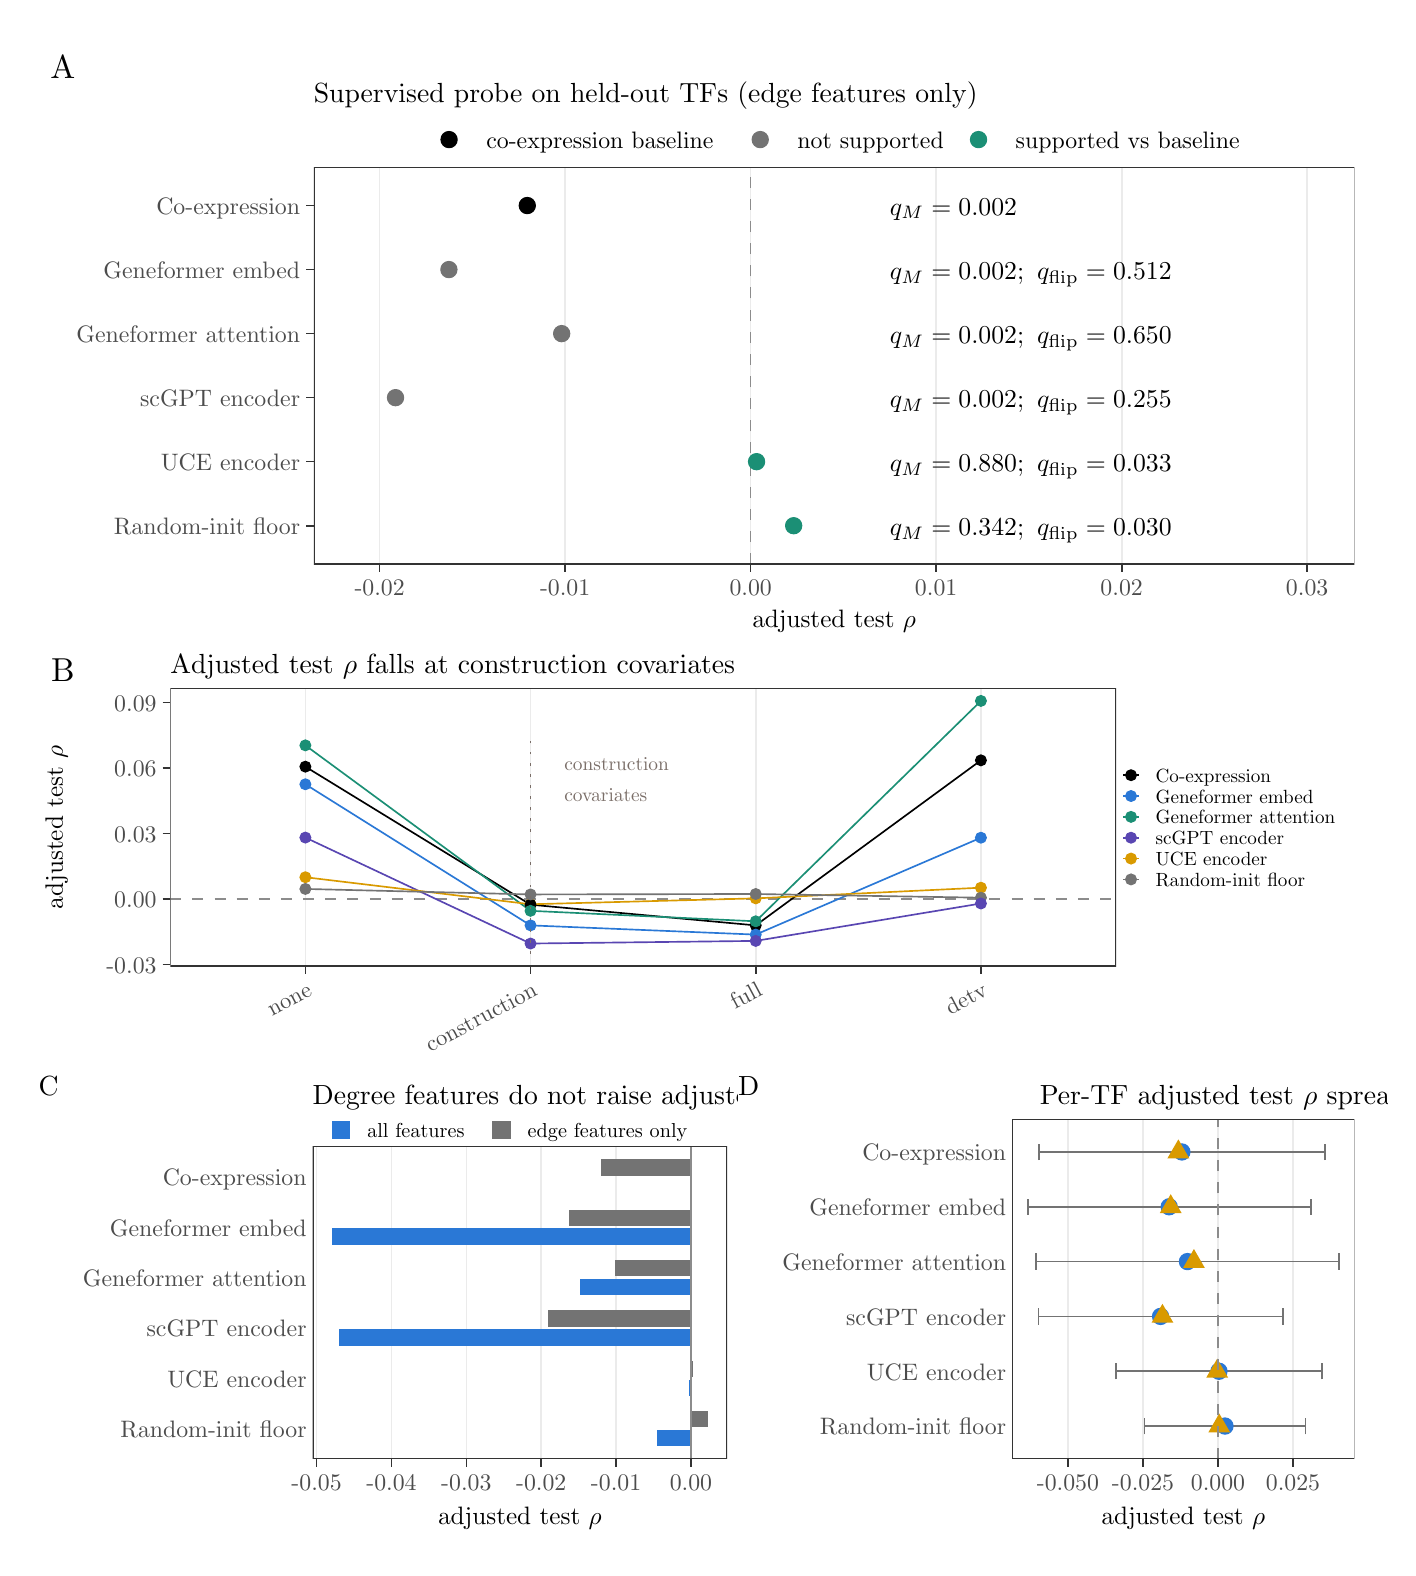
\begin{tikzpicture}[x=1pt,y=1pt]
\definecolor{fillColor}{RGB}{255,255,255}
\path[use as bounding box,fill=fillColor,fill opacity=0.00] (0,0) rectangle (491.44,549.25);
\begin{scope}
\path[clip] (  0.00,  0.00) rectangle (491.44,549.25);
\definecolor{drawColor}{RGB}{255,255,255}
\definecolor{fillColor}{RGB}{255,255,255}

\path[draw=drawColor,line width= 0.6pt,line join=round,line cap=round,fill=fillColor] ( -0.00,  0.00) rectangle (491.44,549.25);
\end{scope}
\begin{scope}
\path[clip] (  4.00,171.71) rectangle (485.44,327.37);
\definecolor{drawColor}{RGB}{255,255,255}
\definecolor{fillColor}{RGB}{255,255,255}

\path[draw=drawColor,line width= 0.6pt,line join=round,line cap=round,fill=fillColor] (  4.00,171.71) rectangle (485.44,327.37);
\end{scope}
\begin{scope}
\path[clip] (  4.00,  3.00) rectangle (485.44,171.71);
\definecolor{drawColor}{RGB}{255,255,255}
\definecolor{fillColor}{RGB}{255,255,255}

\path[draw=drawColor,line width= 0.6pt,line join=round,line cap=round,fill=fillColor] (  4.00,  3.00) rectangle (485.44,171.71);
\end{scope}
\begin{scope}
\path[clip] (  4.00,327.37) rectangle (485.44,545.25);
\definecolor{drawColor}{RGB}{255,255,255}
\definecolor{fillColor}{RGB}{255,255,255}

\path[draw=drawColor,line width= 0.6pt,line join=round,line cap=round,fill=fillColor] (  4.00,327.37) rectangle (485.44,545.25);
\end{scope}
\begin{scope}
\path[clip] (103.39,355.39) rectangle (479.44,498.85);
\definecolor{fillColor}{RGB}{255,255,255}

\path[fill=fillColor] (103.39,355.39) rectangle (479.44,498.85);
\definecolor{drawColor}{gray}{0.92}

\path[draw=drawColor,line width= 0.6pt,line join=round] (127.19,355.39) --
	(127.19,498.85);

\path[draw=drawColor,line width= 0.6pt,line join=round] (194.22,355.39) --
	(194.22,498.85);

\path[draw=drawColor,line width= 0.6pt,line join=round] (261.25,355.39) --
	(261.25,498.85);

\path[draw=drawColor,line width= 0.6pt,line join=round] (328.28,355.39) --
	(328.28,498.85);

\path[draw=drawColor,line width= 0.6pt,line join=round] (395.31,355.39) --
	(395.31,498.85);

\path[draw=drawColor,line width= 0.6pt,line join=round] (462.34,355.39) --
	(462.34,498.85);
\definecolor{drawColor}{gray}{0.55}

\path[draw=drawColor,line width= 0.6pt,dash pattern=on 4pt off 4pt ,line join=round] (261.25,355.39) -- (261.25,498.85);
\definecolor{drawColor}{RGB}{27,143,117}
\definecolor{fillColor}{RGB}{27,143,117}

\path[draw=drawColor,line width= 0.4pt,line join=round,line cap=round,fill=fillColor] (263.38,392.42) circle (  2.93);
\definecolor{drawColor}{RGB}{0,0,0}
\definecolor{fillColor}{RGB}{0,0,0}

\path[draw=drawColor,line width= 0.4pt,line join=round,line cap=round,fill=fillColor] (180.53,484.97) circle (  2.93);
\definecolor{drawColor}{gray}{0.45}
\definecolor{fillColor}{gray}{0.45}

\path[draw=drawColor,line width= 0.4pt,line join=round,line cap=round,fill=fillColor] (192.96,438.69) circle (  2.93);

\path[draw=drawColor,line width= 0.4pt,line join=round,line cap=round,fill=fillColor] (152.21,461.83) circle (  2.93);
\definecolor{drawColor}{RGB}{27,143,117}
\definecolor{fillColor}{RGB}{27,143,117}

\path[draw=drawColor,line width= 0.4pt,line join=round,line cap=round,fill=fillColor] (276.79,369.28) circle (  2.93);
\definecolor{drawColor}{gray}{0.45}
\definecolor{fillColor}{gray}{0.45}

\path[draw=drawColor,line width= 0.4pt,line join=round,line cap=round,fill=fillColor] (132.92,415.55) circle (  2.93);
\definecolor{drawColor}{RGB}{0,0,0}

\node[text=drawColor,anchor=base west,inner sep=0pt, outer sep=0pt, scale=  0.93] at (311.52,388.97) {$q_M=0.880;\ q_{\mathrm{flip}}=0.033$};

\node[text=drawColor,anchor=base west,inner sep=0pt, outer sep=0pt, scale=  0.93] at (311.52,481.52) {$q_M=0.002$};

\node[text=drawColor,anchor=base west,inner sep=0pt, outer sep=0pt, scale=  0.93] at (311.52,435.25) {$q_M=0.002;\ q_{\mathrm{flip}}=0.650$};

\node[text=drawColor,anchor=base west,inner sep=0pt, outer sep=0pt, scale=  0.93] at (311.52,458.38) {$q_M=0.002;\ q_{\mathrm{flip}}=0.512$};

\node[text=drawColor,anchor=base west,inner sep=0pt, outer sep=0pt, scale=  0.93] at (311.52,365.83) {$q_M=0.342;\ q_{\mathrm{flip}}=0.030$};

\node[text=drawColor,anchor=base west,inner sep=0pt, outer sep=0pt, scale=  0.93] at (311.52,412.11) {$q_M=0.002;\ q_{\mathrm{flip}}=0.255$};
\definecolor{drawColor}{gray}{0.20}

\path[draw=drawColor,line width= 0.6pt,line join=round,line cap=round] (103.39,355.39) rectangle (479.44,498.85);
\end{scope}
\begin{scope}
\path[clip] (  0.00,  0.00) rectangle (491.44,549.25);
\definecolor{drawColor}{gray}{0.30}

\node[text=drawColor,anchor=base east,inner sep=0pt, outer sep=0pt, scale=  0.86] at ( 98.44,366.08) {Random-init floor};

\node[text=drawColor,anchor=base east,inner sep=0pt, outer sep=0pt, scale=  0.86] at ( 98.44,389.22) {UCE encoder};

\node[text=drawColor,anchor=base east,inner sep=0pt, outer sep=0pt, scale=  0.86] at ( 98.44,412.36) {scGPT encoder};

\node[text=drawColor,anchor=base east,inner sep=0pt, outer sep=0pt, scale=  0.86] at ( 98.44,435.50) {Geneformer attention};

\node[text=drawColor,anchor=base east,inner sep=0pt, outer sep=0pt, scale=  0.86] at ( 98.44,458.63) {Geneformer embed};

\node[text=drawColor,anchor=base east,inner sep=0pt, outer sep=0pt, scale=  0.86] at ( 98.44,481.77) {Co-expression};
\end{scope}
\begin{scope}
\path[clip] (  0.00,  0.00) rectangle (491.44,549.25);
\definecolor{drawColor}{gray}{0.20}

\path[draw=drawColor,line width= 0.6pt,line join=round] (100.64,369.28) --
	(103.39,369.28);

\path[draw=drawColor,line width= 0.6pt,line join=round] (100.64,392.42) --
	(103.39,392.42);

\path[draw=drawColor,line width= 0.6pt,line join=round] (100.64,415.55) --
	(103.39,415.55);

\path[draw=drawColor,line width= 0.6pt,line join=round] (100.64,438.69) --
	(103.39,438.69);

\path[draw=drawColor,line width= 0.6pt,line join=round] (100.64,461.83) --
	(103.39,461.83);

\path[draw=drawColor,line width= 0.6pt,line join=round] (100.64,484.97) --
	(103.39,484.97);
\end{scope}
\begin{scope}
\path[clip] (  0.00,  0.00) rectangle (491.44,549.25);
\definecolor{drawColor}{gray}{0.20}

\path[draw=drawColor,line width= 0.6pt,line join=round] (127.19,352.64) --
	(127.19,355.39);

\path[draw=drawColor,line width= 0.6pt,line join=round] (194.22,352.64) --
	(194.22,355.39);

\path[draw=drawColor,line width= 0.6pt,line join=round] (261.25,352.64) --
	(261.25,355.39);

\path[draw=drawColor,line width= 0.6pt,line join=round] (328.28,352.64) --
	(328.28,355.39);

\path[draw=drawColor,line width= 0.6pt,line join=round] (395.31,352.64) --
	(395.31,355.39);

\path[draw=drawColor,line width= 0.6pt,line join=round] (462.34,352.64) --
	(462.34,355.39);
\end{scope}
\begin{scope}
\path[clip] (  0.00,  0.00) rectangle (491.44,549.25);
\definecolor{drawColor}{gray}{0.30}

\node[text=drawColor,anchor=base,inner sep=0pt, outer sep=0pt, scale=  0.86] at (127.19,344.05) {-0.02};

\node[text=drawColor,anchor=base,inner sep=0pt, outer sep=0pt, scale=  0.86] at (194.22,344.05) {-0.01};

\node[text=drawColor,anchor=base,inner sep=0pt, outer sep=0pt, scale=  0.86] at (261.25,344.05) {0.00};

\node[text=drawColor,anchor=base,inner sep=0pt, outer sep=0pt, scale=  0.86] at (328.28,344.05) {0.01};

\node[text=drawColor,anchor=base,inner sep=0pt, outer sep=0pt, scale=  0.86] at (395.31,344.05) {0.02};

\node[text=drawColor,anchor=base,inner sep=0pt, outer sep=0pt, scale=  0.86] at (462.34,344.05) {0.03};
\end{scope}
\begin{scope}
\path[clip] (  0.00,  0.00) rectangle (491.44,549.25);
\definecolor{drawColor}{RGB}{0,0,0}

\node[text=drawColor,anchor=base,inner sep=0pt, outer sep=0pt, scale=  0.91] at (291.41,332.53) {adjusted test $\rho$};
\end{scope}
\begin{scope}
\path[clip] (  0.00,  0.00) rectangle (491.44,549.25);
\definecolor{fillColor}{RGB}{255,255,255}

\path[fill=fillColor] (144.32,500.85) rectangle (438.51,516.75);
\end{scope}
\begin{scope}
\path[clip] (  0.00,  0.00) rectangle (491.44,549.25);
\definecolor{fillColor}{RGB}{255,255,255}

\path[fill=fillColor] (144.32,500.85) rectangle (160.22,516.75);
\definecolor{drawColor}{RGB}{0,0,0}
\definecolor{fillColor}{RGB}{0,0,0}

\path[draw=drawColor,line width= 0.4pt,line join=round,line cap=round,fill=fillColor] (152.27,508.80) circle (  2.93);
\end{scope}
\begin{scope}
\path[clip] (  0.00,  0.00) rectangle (491.44,549.25);
\definecolor{fillColor}{RGB}{255,255,255}

\path[fill=fillColor] (256.76,500.85) rectangle (272.66,516.75);
\definecolor{drawColor}{gray}{0.45}
\definecolor{fillColor}{gray}{0.45}

\path[draw=drawColor,line width= 0.4pt,line join=round,line cap=round,fill=fillColor] (264.71,508.80) circle (  2.93);
\end{scope}
\begin{scope}
\path[clip] (  0.00,  0.00) rectangle (491.44,549.25);
\definecolor{fillColor}{RGB}{255,255,255}

\path[fill=fillColor] (335.64,500.85) rectangle (351.54,516.75);
\definecolor{drawColor}{RGB}{27,143,117}
\definecolor{fillColor}{RGB}{27,143,117}

\path[draw=drawColor,line width= 0.4pt,line join=round,line cap=round,fill=fillColor] (343.59,508.80) circle (  2.93);
\end{scope}
\begin{scope}
\path[clip] (  0.00,  0.00) rectangle (491.44,549.25);
\definecolor{drawColor}{RGB}{0,0,0}

\node[text=drawColor,anchor=base west,inner sep=0pt, outer sep=0pt, scale=  0.86] at (165.72,505.61) {co-expression baseline};
\end{scope}
\begin{scope}
\path[clip] (  0.00,  0.00) rectangle (491.44,549.25);
\definecolor{drawColor}{RGB}{0,0,0}

\node[text=drawColor,anchor=base west,inner sep=0pt, outer sep=0pt, scale=  0.86] at (278.16,505.61) {not supported};
\end{scope}
\begin{scope}
\path[clip] (  0.00,  0.00) rectangle (491.44,549.25);
\definecolor{drawColor}{RGB}{0,0,0}

\node[text=drawColor,anchor=base west,inner sep=0pt, outer sep=0pt, scale=  0.86] at (357.04,505.61) {supported vs baseline};
\end{scope}
\begin{scope}
\path[clip] (  0.00,  0.00) rectangle (491.44,549.25);
\definecolor{drawColor}{RGB}{0,0,0}

\node[text=drawColor,anchor=base west,inner sep=0pt, outer sep=0pt, scale=  1.00] at (103.39,522.12) {Supervised probe on held-out TFs (edge features only)};
\end{scope}
\begin{scope}
\path[clip] (  0.00,  0.00) rectangle (491.44,549.25);
\definecolor{drawColor}{RGB}{0,0,0}

\node[text=drawColor,anchor=base,inner sep=0pt, outer sep=0pt, scale=  1.20] at ( 12.74,530.95) {A};
\end{scope}
\begin{scope}
\path[clip] (  4.00,171.71) rectangle (485.44,327.37);
\definecolor{drawColor}{RGB}{255,255,255}
\definecolor{fillColor}{RGB}{255,255,255}

\path[draw=drawColor,line width= 0.6pt,line join=round,line cap=round,fill=fillColor] (  4.00,171.71) rectangle (485.44,327.37);
\end{scope}
\begin{scope}
\path[clip] ( 51.52,210.07) rectangle (393.27,310.54);
\definecolor{fillColor}{RGB}{255,255,255}

\path[fill=fillColor] ( 51.52,210.07) rectangle (393.27,310.54);
\definecolor{drawColor}{gray}{0.92}

\path[draw=drawColor,line width= 0.6pt,line join=round] (100.35,210.07) --
	(100.35,310.54);

\path[draw=drawColor,line width= 0.6pt,line join=round] (181.71,210.07) --
	(181.71,310.54);

\path[draw=drawColor,line width= 0.6pt,line join=round] (263.08,210.07) --
	(263.08,310.54);

\path[draw=drawColor,line width= 0.6pt,line join=round] (344.45,210.07) --
	(344.45,310.54);
\definecolor{drawColor}{gray}{0.55}

\path[draw=drawColor,line width= 0.6pt,dash pattern=on 4pt off 4pt ,line join=round] ( 51.52,234.37) -- (393.27,234.37);
\definecolor{drawColor}{RGB}{0,0,0}

\path[draw=drawColor,line width= 0.6pt,line join=round] (100.35,282.21) --
	(181.71,232.34) --
	(263.08,224.86) --
	(344.45,284.50);
\definecolor{drawColor}{RGB}{42,120,214}

\path[draw=drawColor,line width= 0.6pt,line join=round] (100.35,275.85) --
	(181.71,224.86) --
	(263.08,221.53) --
	(344.45,256.54);
\definecolor{drawColor}{RGB}{27,143,117}

\path[draw=drawColor,line width= 0.6pt,line join=round] (100.35,289.91) --
	(181.71,230.12) --
	(263.08,226.33) --
	(344.45,305.97);
\definecolor{drawColor}{RGB}{89,70,178}

\path[draw=drawColor,line width= 0.6pt,line join=round] (100.35,256.59) --
	(181.71,218.30) --
	(263.08,219.25) --
	(344.45,232.77);
\definecolor{drawColor}{RGB}{217,154,0}

\path[draw=drawColor,line width= 0.6pt,line join=round] (100.35,242.26) --
	(181.71,232.49) --
	(263.08,234.62) --
	(344.45,238.48);
\definecolor{drawColor}{gray}{0.45}

\path[draw=drawColor,line width= 0.6pt,line join=round] (100.35,238.03) --
	(181.71,236.04) --
	(263.08,236.20) --
	(344.45,234.86);
\definecolor{drawColor}{RGB}{217,154,0}
\definecolor{fillColor}{RGB}{217,154,0}

\path[draw=drawColor,line width= 0.4pt,line join=round,line cap=round,fill=fillColor] (181.71,232.49) circle (  1.96);

\path[draw=drawColor,line width= 0.4pt,line join=round,line cap=round,fill=fillColor] (344.45,238.48) circle (  1.96);

\path[draw=drawColor,line width= 0.4pt,line join=round,line cap=round,fill=fillColor] (263.08,234.62) circle (  1.96);

\path[draw=drawColor,line width= 0.4pt,line join=round,line cap=round,fill=fillColor] (100.35,242.26) circle (  1.96);
\definecolor{drawColor}{RGB}{0,0,0}
\definecolor{fillColor}{RGB}{0,0,0}

\path[draw=drawColor,line width= 0.4pt,line join=round,line cap=round,fill=fillColor] (181.71,232.34) circle (  1.96);

\path[draw=drawColor,line width= 0.4pt,line join=round,line cap=round,fill=fillColor] (344.45,284.50) circle (  1.96);

\path[draw=drawColor,line width= 0.4pt,line join=round,line cap=round,fill=fillColor] (263.08,224.86) circle (  1.96);

\path[draw=drawColor,line width= 0.4pt,line join=round,line cap=round,fill=fillColor] (100.35,282.21) circle (  1.96);
\definecolor{drawColor}{RGB}{27,143,117}
\definecolor{fillColor}{RGB}{27,143,117}

\path[draw=drawColor,line width= 0.4pt,line join=round,line cap=round,fill=fillColor] (181.71,230.12) circle (  1.96);

\path[draw=drawColor,line width= 0.4pt,line join=round,line cap=round,fill=fillColor] (344.45,305.97) circle (  1.96);

\path[draw=drawColor,line width= 0.4pt,line join=round,line cap=round,fill=fillColor] (263.08,226.33) circle (  1.96);

\path[draw=drawColor,line width= 0.4pt,line join=round,line cap=round,fill=fillColor] (100.35,289.91) circle (  1.96);
\definecolor{drawColor}{RGB}{42,120,214}
\definecolor{fillColor}{RGB}{42,120,214}

\path[draw=drawColor,line width= 0.4pt,line join=round,line cap=round,fill=fillColor] (181.71,224.86) circle (  1.96);

\path[draw=drawColor,line width= 0.4pt,line join=round,line cap=round,fill=fillColor] (344.45,256.54) circle (  1.96);

\path[draw=drawColor,line width= 0.4pt,line join=round,line cap=round,fill=fillColor] (263.08,221.53) circle (  1.96);

\path[draw=drawColor,line width= 0.4pt,line join=round,line cap=round,fill=fillColor] (100.35,275.85) circle (  1.96);
\definecolor{drawColor}{gray}{0.45}
\definecolor{fillColor}{gray}{0.45}

\path[draw=drawColor,line width= 0.4pt,line join=round,line cap=round,fill=fillColor] (181.71,236.04) circle (  1.96);

\path[draw=drawColor,line width= 0.4pt,line join=round,line cap=round,fill=fillColor] (344.45,234.86) circle (  1.96);

\path[draw=drawColor,line width= 0.4pt,line join=round,line cap=round,fill=fillColor] (263.08,236.20) circle (  1.96);

\path[draw=drawColor,line width= 0.4pt,line join=round,line cap=round,fill=fillColor] (100.35,238.03) circle (  1.96);
\definecolor{drawColor}{RGB}{89,70,178}
\definecolor{fillColor}{RGB}{89,70,178}

\path[draw=drawColor,line width= 0.4pt,line join=round,line cap=round,fill=fillColor] (181.71,218.30) circle (  1.96);

\path[draw=drawColor,line width= 0.4pt,line join=round,line cap=round,fill=fillColor] (344.45,232.77) circle (  1.96);

\path[draw=drawColor,line width= 0.4pt,line join=round,line cap=round,fill=fillColor] (263.08,219.25) circle (  1.96);

\path[draw=drawColor,line width= 0.4pt,line join=round,line cap=round,fill=fillColor] (100.35,256.59) circle (  1.96);
\definecolor{drawColor}{RGB}{122,110,104}

\path[draw=drawColor,line width= 0.5pt,dash pattern=on 1pt off 3pt ,line join=round] (181.71,214.63) -- (181.71,292.00);

\node[text=drawColor,anchor=base west,inner sep=0pt, outer sep=0pt, scale=  0.70] at (193.92,280.74) {construction};

\node[text=drawColor,anchor=base west,inner sep=0pt, outer sep=0pt, scale=  0.70] at (193.92,269.67) {covariates};
\definecolor{drawColor}{gray}{0.20}

\path[draw=drawColor,line width= 0.6pt,line join=round,line cap=round] ( 51.52,210.07) rectangle (393.27,310.54);
\end{scope}
\begin{scope}
\path[clip] (  0.00,  0.00) rectangle (491.44,549.25);
\definecolor{drawColor}{gray}{0.30}

\node[text=drawColor,anchor=base east,inner sep=0pt, outer sep=0pt, scale=  0.86] at ( 46.57,207.49) {-0.03};

\node[text=drawColor,anchor=base east,inner sep=0pt, outer sep=0pt, scale=  0.86] at ( 46.57,231.17) {0.00};

\node[text=drawColor,anchor=base east,inner sep=0pt, outer sep=0pt, scale=  0.86] at ( 46.57,254.86) {0.03};

\node[text=drawColor,anchor=base east,inner sep=0pt, outer sep=0pt, scale=  0.86] at ( 46.57,278.54) {0.06};

\node[text=drawColor,anchor=base east,inner sep=0pt, outer sep=0pt, scale=  0.86] at ( 46.57,302.23) {0.09};
\end{scope}
\begin{scope}
\path[clip] (  0.00,  0.00) rectangle (491.44,549.25);
\definecolor{drawColor}{gray}{0.20}

\path[draw=drawColor,line width= 0.6pt,line join=round] ( 48.77,210.68) --
	( 51.52,210.68);

\path[draw=drawColor,line width= 0.6pt,line join=round] ( 48.77,234.37) --
	( 51.52,234.37);

\path[draw=drawColor,line width= 0.6pt,line join=round] ( 48.77,258.05) --
	( 51.52,258.05);

\path[draw=drawColor,line width= 0.6pt,line join=round] ( 48.77,281.74) --
	( 51.52,281.74);

\path[draw=drawColor,line width= 0.6pt,line join=round] ( 48.77,305.42) --
	( 51.52,305.42);
\end{scope}
\begin{scope}
\path[clip] (  0.00,  0.00) rectangle (491.44,549.25);
\definecolor{drawColor}{gray}{0.20}

\path[draw=drawColor,line width= 0.6pt,line join=round] (100.35,207.32) --
	(100.35,210.07);

\path[draw=drawColor,line width= 0.6pt,line join=round] (181.71,207.32) --
	(181.71,210.07);

\path[draw=drawColor,line width= 0.6pt,line join=round] (263.08,207.32) --
	(263.08,210.07);

\path[draw=drawColor,line width= 0.6pt,line join=round] (344.45,207.32) --
	(344.45,210.07);
\end{scope}
\begin{scope}
\path[clip] (  0.00,  0.00) rectangle (491.44,549.25);
\definecolor{drawColor}{gray}{0.30}

\node[text=drawColor,rotate= 28.00,anchor=base east,inner sep=0pt, outer sep=0pt, scale=  0.82] at (103.19,199.77) {none};

\node[text=drawColor,rotate= 28.00,anchor=base east,inner sep=0pt, outer sep=0pt, scale=  0.82] at (184.56,199.77) {construction};

\node[text=drawColor,rotate= 28.00,anchor=base east,inner sep=0pt, outer sep=0pt, scale=  0.82] at (265.93,199.77) {full};

\node[text=drawColor,rotate= 28.00,anchor=base east,inner sep=0pt, outer sep=0pt, scale=  0.82] at (347.29,199.77) {detv};
\end{scope}
\begin{scope}
\path[clip] (  0.00,  0.00) rectangle (491.44,549.25);
\definecolor{drawColor}{RGB}{0,0,0}

\node[text=drawColor,rotate= 90.00,anchor=base,inner sep=0pt, outer sep=0pt, scale=  0.91] at ( 12.73,260.30) {adjusted test $\rho$};
\end{scope}
\begin{scope}
\path[clip] (  0.00,  0.00) rectangle (491.44,549.25);
\definecolor{fillColor}{RGB}{255,255,255}

\path[fill=fillColor] (395.27,237.71) rectangle (483.44,282.90);
\end{scope}
\begin{scope}
\path[clip] (  0.00,  0.00) rectangle (491.44,549.25);
\definecolor{fillColor}{RGB}{255,255,255}

\path[fill=fillColor] (395.27,275.37) rectangle (402.10,282.90);
\definecolor{drawColor}{RGB}{0,0,0}

\path[draw=drawColor,line width= 0.6pt,line join=round] (395.95,279.13) -- (401.42,279.13);
\definecolor{fillColor}{RGB}{0,0,0}

\path[draw=drawColor,line width= 0.4pt,line join=round,line cap=round,fill=fillColor] (398.69,279.13) circle (  1.96);
\end{scope}
\begin{scope}
\path[clip] (  0.00,  0.00) rectangle (491.44,549.25);
\definecolor{fillColor}{RGB}{255,255,255}

\path[fill=fillColor] (395.27,267.83) rectangle (402.10,275.37);
\definecolor{drawColor}{RGB}{42,120,214}

\path[draw=drawColor,line width= 0.6pt,line join=round] (395.95,271.60) -- (401.42,271.60);
\definecolor{fillColor}{RGB}{42,120,214}

\path[draw=drawColor,line width= 0.4pt,line join=round,line cap=round,fill=fillColor] (398.69,271.60) circle (  1.96);
\end{scope}
\begin{scope}
\path[clip] (  0.00,  0.00) rectangle (491.44,549.25);
\definecolor{fillColor}{RGB}{255,255,255}

\path[fill=fillColor] (395.27,260.30) rectangle (402.10,267.83);
\definecolor{drawColor}{RGB}{27,143,117}

\path[draw=drawColor,line width= 0.6pt,line join=round] (395.95,264.07) -- (401.42,264.07);
\definecolor{fillColor}{RGB}{27,143,117}

\path[draw=drawColor,line width= 0.4pt,line join=round,line cap=round,fill=fillColor] (398.69,264.07) circle (  1.96);
\end{scope}
\begin{scope}
\path[clip] (  0.00,  0.00) rectangle (491.44,549.25);
\definecolor{fillColor}{RGB}{255,255,255}

\path[fill=fillColor] (395.27,252.77) rectangle (402.10,260.30);
\definecolor{drawColor}{RGB}{89,70,178}

\path[draw=drawColor,line width= 0.6pt,line join=round] (395.95,256.54) -- (401.42,256.54);
\definecolor{fillColor}{RGB}{89,70,178}

\path[draw=drawColor,line width= 0.4pt,line join=round,line cap=round,fill=fillColor] (398.69,256.54) circle (  1.96);
\end{scope}
\begin{scope}
\path[clip] (  0.00,  0.00) rectangle (491.44,549.25);
\definecolor{fillColor}{RGB}{255,255,255}

\path[fill=fillColor] (395.27,245.24) rectangle (402.10,252.77);
\definecolor{drawColor}{RGB}{217,154,0}

\path[draw=drawColor,line width= 0.6pt,line join=round] (395.95,249.00) -- (401.42,249.00);
\definecolor{fillColor}{RGB}{217,154,0}

\path[draw=drawColor,line width= 0.4pt,line join=round,line cap=round,fill=fillColor] (398.69,249.00) circle (  1.96);
\end{scope}
\begin{scope}
\path[clip] (  0.00,  0.00) rectangle (491.44,549.25);
\definecolor{fillColor}{RGB}{255,255,255}

\path[fill=fillColor] (395.27,237.71) rectangle (402.10,245.24);
\definecolor{drawColor}{gray}{0.45}

\path[draw=drawColor,line width= 0.6pt,line join=round] (395.95,241.47) -- (401.42,241.47);
\definecolor{fillColor}{gray}{0.45}

\path[draw=drawColor,line width= 0.4pt,line join=round,line cap=round,fill=fillColor] (398.69,241.47) circle (  1.96);
\end{scope}
\begin{scope}
\path[clip] (  0.00,  0.00) rectangle (491.44,549.25);
\definecolor{drawColor}{RGB}{0,0,0}

\node[text=drawColor,anchor=base west,inner sep=0pt, outer sep=0pt, scale=  0.69] at (407.60,276.58) {Co-expression};
\end{scope}
\begin{scope}
\path[clip] (  0.00,  0.00) rectangle (491.44,549.25);
\definecolor{drawColor}{RGB}{0,0,0}

\node[text=drawColor,anchor=base west,inner sep=0pt, outer sep=0pt, scale=  0.69] at (407.60,269.04) {Geneformer embed};
\end{scope}
\begin{scope}
\path[clip] (  0.00,  0.00) rectangle (491.44,549.25);
\definecolor{drawColor}{RGB}{0,0,0}

\node[text=drawColor,anchor=base west,inner sep=0pt, outer sep=0pt, scale=  0.69] at (407.60,261.51) {Geneformer attention};
\end{scope}
\begin{scope}
\path[clip] (  0.00,  0.00) rectangle (491.44,549.25);
\definecolor{drawColor}{RGB}{0,0,0}

\node[text=drawColor,anchor=base west,inner sep=0pt, outer sep=0pt, scale=  0.69] at (407.60,253.98) {scGPT encoder};
\end{scope}
\begin{scope}
\path[clip] (  0.00,  0.00) rectangle (491.44,549.25);
\definecolor{drawColor}{RGB}{0,0,0}

\node[text=drawColor,anchor=base west,inner sep=0pt, outer sep=0pt, scale=  0.69] at (407.60,246.45) {UCE encoder};
\end{scope}
\begin{scope}
\path[clip] (  0.00,  0.00) rectangle (491.44,549.25);
\definecolor{drawColor}{RGB}{0,0,0}

\node[text=drawColor,anchor=base west,inner sep=0pt, outer sep=0pt, scale=  0.69] at (407.60,238.91) {Random-init floor};
\end{scope}
\begin{scope}
\path[clip] (  0.00,  0.00) rectangle (491.44,549.25);
\definecolor{drawColor}{RGB}{0,0,0}

\node[text=drawColor,anchor=base west,inner sep=0pt, outer sep=0pt, scale=  1.00] at ( 51.52,315.97) {Adjusted test $\rho$ falls at construction covariates};
\end{scope}
\begin{scope}
\path[clip] (  0.00,  0.00) rectangle (491.44,549.25);
\definecolor{drawColor}{RGB}{0,0,0}

\node[text=drawColor,anchor=base,inner sep=0pt, outer sep=0pt, scale=  1.20] at ( 12.74,313.07) {B};
\end{scope}
\begin{scope}
\path[clip] (  4.00,  3.00) rectangle (256.75,171.71);
\definecolor{drawColor}{RGB}{255,255,255}
\definecolor{fillColor}{RGB}{255,255,255}

\path[draw=drawColor,line width= 0.6pt,line join=round,line cap=round,fill=fillColor] (  4.00,  3.00) rectangle (256.75,171.71);
\end{scope}
\begin{scope}
\path[clip] (102.99, 32.05) rectangle (252.75,144.91);
\definecolor{fillColor}{RGB}{255,255,255}

\path[fill=fillColor] (102.99, 32.05) rectangle (252.75,144.91);
\definecolor{drawColor}{gray}{0.92}

\path[draw=drawColor,line width= 0.6pt,line join=round] (104.41, 32.05) --
	(104.41,144.91);

\path[draw=drawColor,line width= 0.6pt,line join=round] (131.46, 32.05) --
	(131.46,144.91);

\path[draw=drawColor,line width= 0.6pt,line join=round] (158.51, 32.05) --
	(158.51,144.91);

\path[draw=drawColor,line width= 0.6pt,line join=round] (185.57, 32.05) --
	(185.57,144.91);

\path[draw=drawColor,line width= 0.6pt,line join=round] (212.62, 32.05) --
	(212.62,144.91);

\path[draw=drawColor,line width= 0.6pt,line join=round] (239.67, 32.05) --
	(239.67,144.91);
\definecolor{fillColor}{gray}{0.45}

\path[fill=fillColor] (207.10,134.44) rectangle (239.67,140.36);
\definecolor{fillColor}{RGB}{42,120,214}

\path[fill=fillColor] (239.36,127.62) rectangle (239.67,133.53);
\definecolor{fillColor}{gray}{0.45}

\path[fill=fillColor] (195.66,116.24) rectangle (239.67,122.15);
\definecolor{fillColor}{RGB}{42,120,214}

\path[fill=fillColor] (109.80,109.41) rectangle (239.67,115.33);
\definecolor{fillColor}{gray}{0.45}

\path[fill=fillColor] (212.11, 98.04) rectangle (239.67,103.95);
\definecolor{fillColor}{RGB}{42,120,214}

\path[fill=fillColor] (199.56, 91.21) rectangle (239.67, 97.13);
\definecolor{fillColor}{gray}{0.45}

\path[fill=fillColor] (187.88, 79.83) rectangle (239.67, 85.75);
\definecolor{fillColor}{RGB}{42,120,214}

\path[fill=fillColor] (112.63, 73.01) rectangle (239.67, 78.92);
\definecolor{fillColor}{gray}{0.45}

\path[fill=fillColor] (239.67, 61.63) rectangle (240.53, 67.55);
\definecolor{fillColor}{RGB}{42,120,214}

\path[fill=fillColor] (238.79, 54.81) rectangle (239.67, 60.72);
\definecolor{fillColor}{gray}{0.45}

\path[fill=fillColor] (239.67, 43.43) rectangle (245.95, 49.35);
\definecolor{fillColor}{RGB}{42,120,214}

\path[fill=fillColor] (227.48, 36.60) rectangle (239.67, 42.52);
\definecolor{drawColor}{gray}{0.55}

\path[draw=drawColor,line width= 0.6pt,line join=round] (239.67, 32.05) -- (239.67,144.91);
\definecolor{drawColor}{gray}{0.20}

\path[draw=drawColor,line width= 0.6pt,line join=round,line cap=round] (102.99, 32.05) rectangle (252.75,144.91);
\end{scope}
\begin{scope}
\path[clip] (  0.00,  0.00) rectangle (491.44,549.25);
\definecolor{drawColor}{gray}{0.30}

\node[text=drawColor,anchor=base east,inner sep=0pt, outer sep=0pt, scale=  0.86] at (100.79, 39.78) {Random-init floor};

\node[text=drawColor,anchor=base east,inner sep=0pt, outer sep=0pt, scale=  0.86] at (100.79, 57.98) {UCE encoder};

\node[text=drawColor,anchor=base east,inner sep=0pt, outer sep=0pt, scale=  0.86] at (100.79, 76.18) {scGPT encoder};

\node[text=drawColor,anchor=base east,inner sep=0pt, outer sep=0pt, scale=  0.86] at (100.79, 94.39) {Geneformer attention};

\node[text=drawColor,anchor=base east,inner sep=0pt, outer sep=0pt, scale=  0.86] at (100.79,112.59) {Geneformer embed};

\node[text=drawColor,anchor=base east,inner sep=0pt, outer sep=0pt, scale=  0.86] at (100.79,130.79) {Co-expression};
\end{scope}
\begin{scope}
\path[clip] (  0.00,  0.00) rectangle (491.44,549.25);
\definecolor{drawColor}{gray}{0.20}

\path[draw=drawColor,line width= 0.6pt,line join=round] (104.41, 29.30) --
	(104.41, 32.05);

\path[draw=drawColor,line width= 0.6pt,line join=round] (131.46, 29.30) --
	(131.46, 32.05);

\path[draw=drawColor,line width= 0.6pt,line join=round] (158.51, 29.30) --
	(158.51, 32.05);

\path[draw=drawColor,line width= 0.6pt,line join=round] (185.57, 29.30) --
	(185.57, 32.05);

\path[draw=drawColor,line width= 0.6pt,line join=round] (212.62, 29.30) --
	(212.62, 32.05);

\path[draw=drawColor,line width= 0.6pt,line join=round] (239.67, 29.30) --
	(239.67, 32.05);
\end{scope}
\begin{scope}
\path[clip] (  0.00,  0.00) rectangle (491.44,549.25);
\definecolor{drawColor}{gray}{0.30}

\node[text=drawColor,anchor=base,inner sep=0pt, outer sep=0pt, scale=  0.86] at (104.41, 20.71) {-0.05};

\node[text=drawColor,anchor=base,inner sep=0pt, outer sep=0pt, scale=  0.86] at (131.46, 20.71) {-0.04};

\node[text=drawColor,anchor=base,inner sep=0pt, outer sep=0pt, scale=  0.86] at (158.51, 20.71) {-0.03};

\node[text=drawColor,anchor=base,inner sep=0pt, outer sep=0pt, scale=  0.86] at (185.57, 20.71) {-0.02};

\node[text=drawColor,anchor=base,inner sep=0pt, outer sep=0pt, scale=  0.86] at (212.62, 20.71) {-0.01};

\node[text=drawColor,anchor=base,inner sep=0pt, outer sep=0pt, scale=  0.86] at (239.67, 20.71) {0.00};
\end{scope}
\begin{scope}
\path[clip] (  0.00,  0.00) rectangle (491.44,549.25);
\definecolor{drawColor}{RGB}{0,0,0}

\node[text=drawColor,anchor=base,inner sep=0pt, outer sep=0pt, scale=  0.91] at (177.87,  8.21) {adjusted test $\rho$};
\end{scope}
\begin{scope}
\path[clip] (  0.00,  0.00) rectangle (491.44,549.25);
\definecolor{fillColor}{RGB}{255,255,255}

\path[fill=fillColor] (109.23,146.91) rectangle (246.52,154.87);
\end{scope}
\begin{scope}
\path[clip] (  0.00,  0.00) rectangle (491.44,549.25);
\definecolor{fillColor}{RGB}{255,255,255}

\path[fill=fillColor] (109.23,146.91) rectangle (117.20,154.87);
\definecolor{fillColor}{RGB}{42,120,214}

\path[fill=fillColor] (109.94,147.62) rectangle (116.48,154.16);
\end{scope}
\begin{scope}
\path[clip] (  0.00,  0.00) rectangle (491.44,549.25);
\definecolor{fillColor}{RGB}{255,255,255}

\path[fill=fillColor] (167.23,146.91) rectangle (175.20,154.87);
\definecolor{fillColor}{gray}{0.45}

\path[fill=fillColor] (167.94,147.62) rectangle (174.49,154.16);
\end{scope}
\begin{scope}
\path[clip] (  0.00,  0.00) rectangle (491.44,549.25);
\definecolor{drawColor}{RGB}{0,0,0}

\node[text=drawColor,anchor=base west,inner sep=0pt, outer sep=0pt, scale=  0.73] at (122.70,148.20) {all features};
\end{scope}
\begin{scope}
\path[clip] (  0.00,  0.00) rectangle (491.44,549.25);
\definecolor{drawColor}{RGB}{0,0,0}

\node[text=drawColor,anchor=base west,inner sep=0pt, outer sep=0pt, scale=  0.73] at (180.70,148.20) {edge features only};
\end{scope}
\begin{scope}
\path[clip] (  0.00,  0.00) rectangle (491.44,549.25);
\definecolor{drawColor}{RGB}{0,0,0}

\node[text=drawColor,anchor=base west,inner sep=0pt, outer sep=0pt, scale=  1.00] at (102.99,160.30) {Degree features do not raise adjusted test $\rho$};
\end{scope}
\begin{scope}
\path[clip] (  0.00,  0.00) rectangle (491.44,549.25);
\definecolor{drawColor}{RGB}{0,0,0}

\node[text=drawColor,anchor=base west,inner sep=0pt, outer sep=0pt, scale=  1.00] at (  4.00,163.56) {C};
\end{scope}
\begin{scope}
\path[clip] (256.75,  3.00) rectangle (485.44,171.71);
\definecolor{drawColor}{RGB}{255,255,255}
\definecolor{fillColor}{RGB}{255,255,255}

\path[draw=drawColor,line width= 0.6pt,line join=round,line cap=round,fill=fillColor] (256.75,  3.00) rectangle (485.44,171.71);
\end{scope}
\begin{scope}
\path[clip] (355.75, 32.05) rectangle (479.44,154.87);
\definecolor{fillColor}{RGB}{255,255,255}

\path[fill=fillColor] (355.75, 32.05) rectangle (479.44,154.87);
\definecolor{drawColor}{gray}{0.92}

\path[draw=drawColor,line width= 0.6pt,line join=round] (375.91, 32.05) --
	(375.91,154.87);

\path[draw=drawColor,line width= 0.6pt,line join=round] (403.02, 32.05) --
	(403.02,154.87);

\path[draw=drawColor,line width= 0.6pt,line join=round] (430.13, 32.05) --
	(430.13,154.87);

\path[draw=drawColor,line width= 0.6pt,line join=round] (457.24, 32.05) --
	(457.24,154.87);
\definecolor{drawColor}{gray}{0.45}

\path[draw=drawColor,line width= 0.6pt,line join=round] (468.76,140.02) --
	(468.76,145.96);

\path[draw=drawColor,line width= 0.6pt,line join=round] (468.76,142.99) --
	(365.38,142.99);

\path[draw=drawColor,line width= 0.6pt,line join=round] (365.38,140.02) --
	(365.38,145.96);

\path[draw=drawColor,line width= 0.6pt,line join=round] (463.61,120.21) --
	(463.61,126.15);

\path[draw=drawColor,line width= 0.6pt,line join=round] (463.61,123.18) --
	(361.37,123.18);

\path[draw=drawColor,line width= 0.6pt,line join=round] (361.37,120.21) --
	(361.37,126.15);

\path[draw=drawColor,line width= 0.6pt,line join=round] (473.81,100.40) --
	(473.81,106.34);

\path[draw=drawColor,line width= 0.6pt,line join=round] (473.81,103.37) --
	(364.35,103.37);

\path[draw=drawColor,line width= 0.6pt,line join=round] (364.35,100.40) --
	(364.35,106.34);

\path[draw=drawColor,line width= 0.6pt,line join=round] (453.52, 80.59) --
	(453.52, 86.53);

\path[draw=drawColor,line width= 0.6pt,line join=round] (453.52, 83.56) --
	(365.22, 83.56);

\path[draw=drawColor,line width= 0.6pt,line join=round] (365.22, 80.59) --
	(365.22, 86.53);

\path[draw=drawColor,line width= 0.6pt,line join=round] (467.73, 60.78) --
	(467.73, 66.72);

\path[draw=drawColor,line width= 0.6pt,line join=round] (467.73, 63.75) --
	(393.22, 63.75);

\path[draw=drawColor,line width= 0.6pt,line join=round] (393.22, 60.78) --
	(393.22, 66.72);

\path[draw=drawColor,line width= 0.6pt,line join=round] (461.73, 40.97) --
	(461.73, 46.91);

\path[draw=drawColor,line width= 0.6pt,line join=round] (461.73, 43.94) --
	(403.56, 43.94);

\path[draw=drawColor,line width= 0.6pt,line join=round] (403.56, 40.97) --
	(403.56, 46.91);
\definecolor{drawColor}{RGB}{42,120,214}
\definecolor{fillColor}{RGB}{42,120,214}

\path[draw=drawColor,line width= 0.4pt,line join=round,line cap=round,fill=fillColor] (417.07,142.99) circle (  2.93);

\path[draw=drawColor,line width= 0.4pt,line join=round,line cap=round,fill=fillColor] (412.49,123.18) circle (  2.93);

\path[draw=drawColor,line width= 0.4pt,line join=round,line cap=round,fill=fillColor] (419.08,103.37) circle (  2.93);

\path[draw=drawColor,line width= 0.4pt,line join=round,line cap=round,fill=fillColor] (409.37, 83.56) circle (  2.93);

\path[draw=drawColor,line width= 0.4pt,line join=round,line cap=round,fill=fillColor] (430.47, 63.75) circle (  2.93);

\path[draw=drawColor,line width= 0.4pt,line join=round,line cap=round,fill=fillColor] (432.64, 43.94) circle (  2.93);
\definecolor{fillColor}{RGB}{217,154,0}

\path[fill=fillColor] (415.80,147.54) --
	(419.74,140.71) --
	(411.86,140.71) --
	cycle;

\path[fill=fillColor] (413.03,127.73) --
	(416.97,120.90) --
	(409.09,120.90) --
	cycle;

\path[fill=fillColor] (421.42,107.92) --
	(425.36,101.09) --
	(417.48,101.09) --
	cycle;

\path[fill=fillColor] (410.05, 88.11) --
	(414.00, 81.28) --
	(406.11, 81.28) --
	cycle;

\path[fill=fillColor] (429.83, 68.30) --
	(433.77, 61.47) --
	(425.89, 61.47) --
	cycle;

\path[fill=fillColor] (430.58, 48.49) --
	(434.52, 41.66) --
	(426.64, 41.66) --
	cycle;
\definecolor{drawColor}{gray}{0.55}

\path[draw=drawColor,line width= 0.6pt,dash pattern=on 4pt off 4pt ,line join=round] (430.13, 32.05) -- (430.13,154.87);
\definecolor{drawColor}{gray}{0.20}

\path[draw=drawColor,line width= 0.6pt,line join=round,line cap=round] (355.75, 32.05) rectangle (479.44,154.87);
\end{scope}
\begin{scope}
\path[clip] (  0.00,  0.00) rectangle (491.44,549.25);
\definecolor{drawColor}{gray}{0.30}

\node[text=drawColor,anchor=base east,inner sep=0pt, outer sep=0pt, scale=  0.86] at (353.55, 40.74) {Random-init floor};

\node[text=drawColor,anchor=base east,inner sep=0pt, outer sep=0pt, scale=  0.86] at (353.55, 60.55) {UCE encoder};

\node[text=drawColor,anchor=base east,inner sep=0pt, outer sep=0pt, scale=  0.86] at (353.55, 80.36) {scGPT encoder};

\node[text=drawColor,anchor=base east,inner sep=0pt, outer sep=0pt, scale=  0.86] at (353.55,100.17) {Geneformer attention};

\node[text=drawColor,anchor=base east,inner sep=0pt, outer sep=0pt, scale=  0.86] at (353.55,119.98) {Geneformer embed};

\node[text=drawColor,anchor=base east,inner sep=0pt, outer sep=0pt, scale=  0.86] at (353.55,139.79) {Co-expression};
\end{scope}
\begin{scope}
\path[clip] (  0.00,  0.00) rectangle (491.44,549.25);
\definecolor{drawColor}{gray}{0.20}

\path[draw=drawColor,line width= 0.6pt,line join=round] (375.91, 29.30) --
	(375.91, 32.05);

\path[draw=drawColor,line width= 0.6pt,line join=round] (403.02, 29.30) --
	(403.02, 32.05);

\path[draw=drawColor,line width= 0.6pt,line join=round] (430.13, 29.30) --
	(430.13, 32.05);

\path[draw=drawColor,line width= 0.6pt,line join=round] (457.24, 29.30) --
	(457.24, 32.05);
\end{scope}
\begin{scope}
\path[clip] (  0.00,  0.00) rectangle (491.44,549.25);
\definecolor{drawColor}{gray}{0.30}

\node[text=drawColor,anchor=base,inner sep=0pt, outer sep=0pt, scale=  0.86] at (375.91, 20.71) {-0.050};

\node[text=drawColor,anchor=base,inner sep=0pt, outer sep=0pt, scale=  0.86] at (403.02, 20.71) {-0.025};

\node[text=drawColor,anchor=base,inner sep=0pt, outer sep=0pt, scale=  0.86] at (430.13, 20.71) {0.000};

\node[text=drawColor,anchor=base,inner sep=0pt, outer sep=0pt, scale=  0.86] at (457.24, 20.71) {0.025};
\end{scope}
\begin{scope}
\path[clip] (  0.00,  0.00) rectangle (491.44,549.25);
\definecolor{drawColor}{RGB}{0,0,0}

\node[text=drawColor,anchor=base,inner sep=0pt, outer sep=0pt, scale=  0.91] at (417.59,  8.21) {adjusted test $\rho$};
\end{scope}
\begin{scope}
\path[clip] (  0.00,  0.00) rectangle (491.44,549.25);
\definecolor{drawColor}{RGB}{0,0,0}

\node[text=drawColor,anchor=base west,inner sep=0pt, outer sep=0pt, scale=  1.00] at (365.75,160.30) {Per-TF adjusted test $\rho$ spread};
\end{scope}
\begin{scope}
\path[clip] (  0.00,  0.00) rectangle (491.44,549.25);
\definecolor{drawColor}{RGB}{0,0,0}

\node[text=drawColor,anchor=base west,inner sep=0pt, outer sep=0pt, scale=  1.00] at (256.75,163.56) {D};
\end{scope}
\end{tikzpicture}
